\documentclass[svgnames]{beamer}
\usepackage{graphicx}
\usepackage{xcolor}
\usepackage{tikz}
\usepackage{tikzscale}
\usetikzlibrary{positioning}
\usepackage{filecontents}
\usepackage{multicol}
\usepackage[export]{adjustbox}
\usepackage{tcolorbox}

\usetheme{Boadilla}
\usecolortheme{dolphin}
\graphicspath{{fig/}}

% change text to offblack
\definecolor{almostblack}{HTML}{262626}
\setbeamercolor{normal text}{fg=almostblack}
\definecolor{pyred}{HTML}{DA2623}
\definecolor{pyblue}{HTML}{2E7EBC}

\title[DIS]{Probing the structure of hadrons \\with deep inelastic scattering (DIS)}
\author[Scott Moreland]{Scott Moreland $\vert$ \today}
\date[\today]{} 

\begin{document}

\begin{frame}
    \maketitle
\end{frame}

\begin{frame}{Deep inelastic scattering (DIS)}

\begin{columns}
\begin{column}{0.05\textwidth}
\end{column}
\begin{column}{0.55\textwidth}
In DIS a charged lepton $\ell^{\pm}$ scatters off a hadron, e.g.\ electron-proton scattering, and exchanges momentum $q$ with a struck parton in the nucleon.
\end{column}
\begin{column}{0.35\textwidth}
    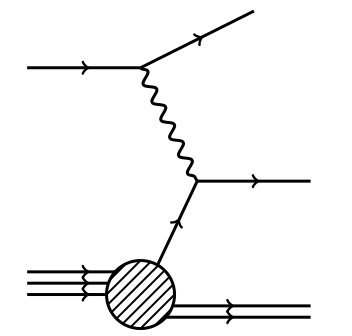
\includegraphics[width=0.9\columnwidth]{dis}
\end{column}
\end{columns}

\begin{itemize}
    \item label initial and final electron momentum $k$ and $k'$
    \item final electron deflected $q = k - k'$ by virtual photon $\gamma$
    \item momentum transfer conventionally expressed using $Q^2 = -q^2$
\end{itemize}
\bigskip
For large $Q^2$, the parton is ejected from the target nucleon and produces a shower of gluons and quark/anti-quark pairs, hence the name deep \emph{inelastic} scattering.
\vfill
\end{frame}

\begin{frame}{Partonic description of the proton}
Consider high-energy electron-proton CMS frame where $m_\text{proton} \ll \sqrt{s}$ \\
Proton and its constituents have lightlike momenta \bigskip \\
Running $\alpha_s$ coupling suppresses hard gluon exchange inside proton, hence constinuents have small transverse momentum relative to longitudinal momentum, i.e.\ partons are collinear with proton \bigskip \\

To leading order in pQCD, parton momentum $p = x P$, \\
where $x \in \{0, 1\}$ is fraction of proton momentum $P$ \bigskip\\

To leading order in $\alpha_s$, gluons contributions negligible and cross section for electron-proton scattering is
\small
\begin{equation*}
    \sigma(e^-(k) p(P) \rightarrow e^-(k') + X) = \int\limits_0^1 dx \sum\limits_f f_f(x)\, \sigma(e^-(k) q_f(x P) \rightarrow e^-(k') q_f(p'))
\end{equation*}

\footnote{Next few slides based on Peskin}
\end{frame}

\begin{frame}{Working out the leading-order cross section}

Here $f_f(x) dx$ is probability of finding a parton $f$ in the proton with momentum fraction $x$. Parton model includes sea quarks as well as constituent quarks. \bigskip\\

The pQCD matrix amplitude for electron-quark scattering for massless quarks is,
\begin{equation*}
    \frac{1}{4} \sum\limits_\text{spins} |\mathcal{M}|^2 = \frac{8 e^4 Q_i^2}{\hat{t}^2} \Big(\frac{\hat{s}^2 + \hat{u}^2}{4}  \Big)
\end{equation*}
from which it can be shown that,
\begin{equation*}
    \frac{d\sigma}{d\hat{t}} = \frac{2\pi \alpha^2 Q_i^2}{\hat{s}^2} \Big( \frac{\hat{s}^2 + (\hat{s}+\hat{t})^2}{\hat{t}^2} \Big)
\end{equation*}
\end{frame}

\begin{frame}{Working out the leading-order cross section}

    Starting from the pQCD differential cross section (below), one can express Mandelstam $\hat{t}$ and $\hat{s}$ in terms of experimental quantities. 
    \begin{equation*}
        \frac{d\sigma}{d\hat{t}} = \frac{2\pi \alpha^2 Q_i^2}{\hat{s}^2} \Big( \frac{\hat{s}^2 + (\hat{s}+\hat{t})^2}{\hat{t}^2} \Big)
    \end{equation*} \\
    \medskip For example, it's easy to identify $\hat{t}=-Q^2$. To re-express Mandelstam $\hat{s}$, note that in the massless limit, 
    \begin{equation*}
        \hat{s} = (p + k)^2 = 2 p \cdot k = 2 x P \cdot k = x\, s
    \end{equation*}
    where $p$ and $k$ are the initial parton and electron momentum respectively. \bigskip \\
    Hence the electron-parton collision carries a fraction $\hat{s} = x\, s$ of the total proton-electron CMS collision energy
\end{frame}

\begin{frame}{Working out the leading-order cross section}
To briefly summarize, the electron-quark differential cross section is given below, 
    \begin{equation}
        \label{differential}
        \frac{d\sigma}{d\hat{t}} = \frac{2\pi \alpha^2 Q_i^2}{\hat{s}^2} \Big( \frac{\hat{s}^2 + (\hat{s}+\hat{t})^2}{\hat{t}^2} \Big)
    \end{equation} \\
    where $\hat{t} = -Q^2$ and $\hat{s} = x\, s$. It turns out we can measure $x$ from the electron momentum alone and hence experimentally test Eq.~\eqref{differential}. \bigskip \\

  To see this, note that the scattered quark in the proton acquires momentum $p' = p+q$ where $q$ is the virtual photon momentum. This quark is also "massless" which implies $(p + q)^2 \approx 0$ and thus, \\
\begin{equation*}
    0 \approx (p+q)^2 = 2p \cdot q + q^2 = 2xP \cdot q - Q^2
\end{equation*}
Solving for $x$ one finds that $x \equiv Q^2 / (2 P \cdot q)$ which can be used to specify Eq.\eqref{differential} in terms of measureables $s$, $P$, $Q$ and $q$.

\end{frame}

\begin{frame}{Working out the leading-order cross section}
    We can now express the electron-proton cross section $\sigma(e^-(k) p(P) \rightarrow e^-(k') + X)$ in the new coordinates $x$ and $Q^2$,
\begin{equation}
    \label{dsdxdQ2}
    \frac{d^2\sigma}{dx\, dQ^2} = \sum\limits_i f_i(x) Q_i^2 \cdot \frac{2 \pi \alpha^2}{Q^4} \Bigg[ 1 + \Bigg(1-\frac{Q^2}{x\, s} \Bigg)^2 \Bigg].
\end{equation}

The parton distribution functions $f_i$ depend only on the details of the proton, cannot be calculated from first principles and are determined from experiment. \bigskip \\

However, if we divide Eq.\eqref{dsdxdQ2} by the factor,\\
\begin{equation*}
    \frac{1 + (1 - Q^2/x\, s)^2}{Q^4}
\end{equation*}
then Eq.~\eqref{dsdxdQ2} \emph{depends only on $x$ and is independent of $Q^2$!} This is a non-trivial prediction which can be validated by experiment.
\end{frame}

\begin{frame}{Experimental validation of Bjorken scaling}
    \begin{columns}
    \begin{column}{0.455\textwidth}
        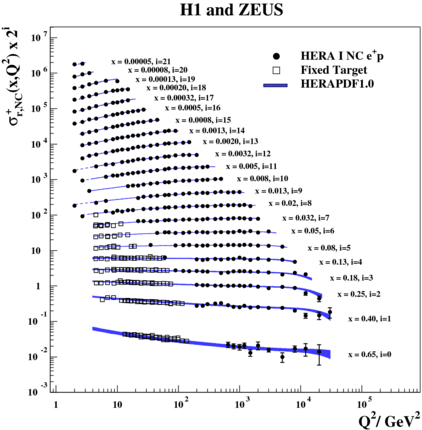
\includegraphics[width=\columnwidth]{structure_func}
    \end{column}
    \begin{column}{0.025\textwidth}
    \end{column}
    \begin{column}{0.455\textwidth}
        DIS experiments were originally performed at SLAC in the 60's. Modern DIS experiments, performed at HERA in Germany, allow broad range in $Q^2$ and $x$. HERA collides 920 GeV protons off 27.5 GeV electrons with $\sqrt{s} \gg 320$ GeV! \medskip \\ 
        Bjorken scaling evidenced by near flatness of the reduced electron-proton cross section as a function of $Q^2$ (left figure). 
    \end{column}
    \begin{column}{0.025\textwidth}
    \end{column}
    \end{columns}
    \medskip
    Important takeaway: proton looks the same to an electromagnetic probe no matter how much momentum is exchanged!
\end{frame}

\begin{frame}{DIS established the quarks as real entities}
    SU(3) was introduced as a mathematical tool by Gell-Mann and Ne'eman in 1961, and later the concept of quarks by Gell-Mann and Zweig. \bigskip\\

    Idea of fractional charges not well accepted at the time and even Gell-Mann wrote, "the search for stable quarks at the highest accelerator energies would help reassure us of the non-existence of real quarks" \bigskip\\

    However, initial DIS experiments showed the electron rebounded with far less energy than expected after striking the proton. Even after correcting for radiative energy loss, the tension remained. \bigskip \\

   Partonic description of proton emerged - revelation which paralleled Rutherford's discovery of nuclear structure. Formally proposed by Feynman, although initially did not describe the quantum numbers of the partons. 

\end{frame}

\begin{frame}{Parton distribution functions}
    \begin{columns}
    \begin{column}{0.5\textwidth}
        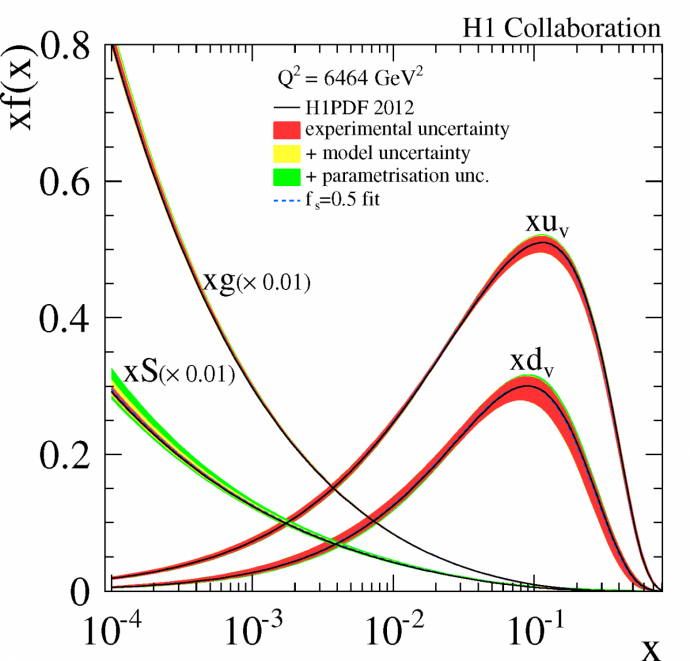
\includegraphics[width=\columnwidth]{PDF}
    \end{column}
    \begin{column}{0.5\textwidth}
    The sets of measured cross sections can then be used to determine the parton distribution functions (left) \bigskip \\
    Note the gluons and sea quarks dominate the PDF at small-x and there is a 2-to-1 ratio of u quarks to d quarks at large-x in the proton \bigskip \\
    Moreover the PDF's obey: \\
    $\int_0^1 dx [f_u(x) - f_{\bar{u}}(x)] = 2$ \\
    $\int_0^1 dx [f_d(x) - f_{\bar{d}}(x)] = 1$ \\
    \end{column}
    \end{columns}
    \bigskip \centering
    and $\int\limits_0^1 dx\, x[f_u(x) + f_d(x) + f_{\bar{u}}(x) + f_{\bar{d}} + f_g(x)] = 1$
\end{frame}

\begin{frame}{Spatial distribution of partons inside the proton}
Size of the proton depends on what you measure... \bigskip \\
Proton \emph{charge} radius can be determined from elastic electron-proton scattering using the Born approximation,
\begin{align*}
    \cr G_E(Q^2) &= 1 - \frac{Q^2}{6} \langle r^2 \rangle + \frac{Q^2}{120} \langle r^4 \rangle + ... \\
    r_\text{rms} &= -6 \frac{\partial G_E(Q^2)}{\partial (Q^2)} \Bigg\vert_{Q^2=0}
\end{align*}
The rms charge radius is $r_\text{rms} \approx 0.85 -0.9$ fm depending who you ask. \bigskip \\

But what about charge neutral gluons? How are quarks and gluons spatially distributed in the proton?
\end{frame}

\begin{frame}{Using DIS to size the gluon cloud radius}
\bigskip
In the color-dipole model, the virtual photon $\gamma^*$ interacts with the proton by fluctuating into a $q \bar{q}$ pair
\begin{equation*}
    \sigma^{\gamma^* p}_{L,T}(Q^2, x) = 2 \sum\limits_f \int \int d^2b\, d^2r \int\limits_0^1 dz | \Psi^{(f)}_{L,T}(r,z;Q^2)|^2 \mathcal{N}(x,r,b)
\end{equation*}
Here $\Psi^{(f)}_{L,T}$ is the lightcone wavefunction for $\gamma^* \rightarrow q\bar{q}$ fluctuations \\
$\mathcal{N}(x,r,b)$ is the imaginary part of the forward scattering amplitude \bigskip \\

The reduced cross section $\sigma_r$, which is directly measureable, can then be expressed as functions of the proton structure functions $F_2$ and $F_L$ which depend on  $\sigma^{\gamma^* p}_{L}$ and $\sigma^{\gamma^* p}_{T}$.  
\begin{equation*}
    \sigma_r(x,y,Q^2) = F_2(x,Q^2) - \frac{y^2}{1 + (1-y)^2} F_L(x, Q^2)
\end{equation*}

\end{frame}

\begin{frame}{Using DIS to size the gluon cloud radius}
    In the IP-Sat model [Rezaeian, et.\ al.\, Phys.Rev.D87, 2013] of color-dipole DIS, the forward scattering amplitude is parameterized using the form, \\
    \begin{equation*}
    \mathcal{N}(x,r,b) = \Bigg(1 - \exp\Bigg(-\frac{\pi^2 r^2}{2 N_c} \alpha_s(\mu^2) xg(x, \mu^2) T_G(b) \Bigg) \Bigg)
    \end{equation*}
    with Gaussian impact parameter profile,
    \begin{equation*}
        T_G(b) = \frac{1}{2 \pi B_G} \exp(-b^2/2 B_G).
    \end{equation*}
    The initial gluon distribution at momentum scale $\mu_0^2$ is parameterized by, \\
    \begin{equation*}
        x g(x, \mu_0^2) = A_g x^{-\lambda_g} (1 - x)^{5.6}.
    \end{equation*}
    The parameters $A_g$, $\lambda_g$, $\mu_0^2$ and $B_G$ are then tuned by a fit to the reduced cross sections $\sigma_r$.
\end{frame}
\begin{frame}{Using DIS to size the gluon cloud radius}

The IP-Sat model for color-dipole DIS, once tuned to fit the reduced cross sections $\sigma_r$ for different values of $Q^2$ and $x$, finds a gluon distribution in the proton of width $B_G \approx 4$~GeV$^{-2}$ corresponding to Gaussian width $r^\text{gluon}_\text{rms} \approx 0.4$~fm. \bigskip \\

This is about half the proton charge radius $r^\text{chg}_\text{rms} \approx 0.85-0.9$~fm! \bigskip \\

Physical picture: gluons are self interacting, tightly clustered inside charge density distribution \bigskip \\

Inerestingly, the proton width also enters in hydrodynamic simulations of relativistic heavy-ion collisions. Sets the scale of proton-proton "hot spots" in the collision which drive collective flow.  
\end{frame}

\usebackgroundtemplate{%
\tikz[overlay,remember picture] \node[at=(current page.center)] {
   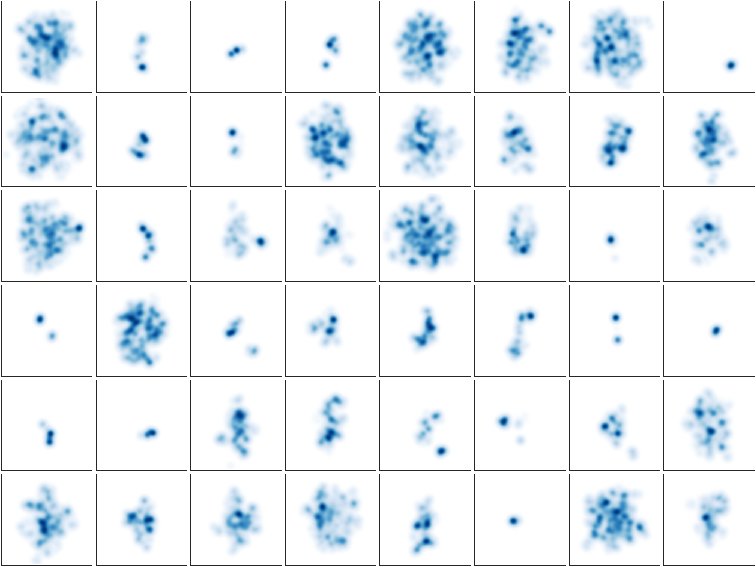
\includegraphics[width=\paperwidth]{trento_minbias}};
}

\setbeamertemplate{footline}[frame number]{}
\setbeamertemplate{navigation symbols}{}
\setbeamertemplate{footline}{}

\begin{frame}
\end{frame}
\usebackgroundtemplate{}

\begin{frame}
    \begin{columns}
        \begin{column}{1 cm}
            \centering
            \hspace{0.5 cm}
            \rotatebox[origin=c]{90}{\scriptsize \only<1>{\color{pyblue}} 
            \only<2->{\color{pyblue!40}} Calibrated to identified particles}
        \end{column}
        \begin{column}{\paperheight}
            \centering \vspace{0.3 cm}\\
            \begin{tikzpicture}
                \only<1>{\node [opacity=1] (post) {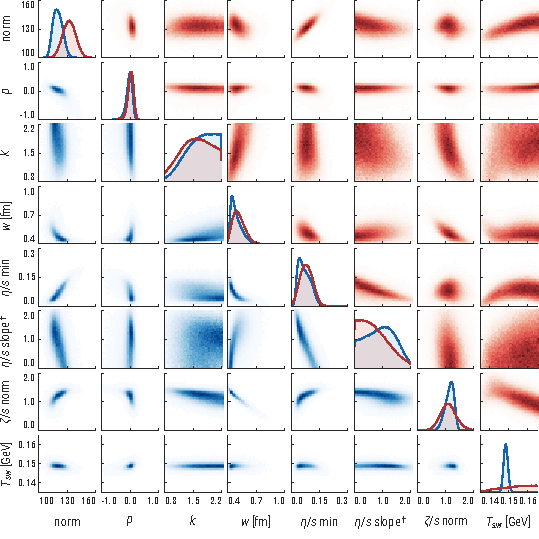
\includegraphics{posterior}};}
                \only<2->{\node [opacity=0.3] (post) {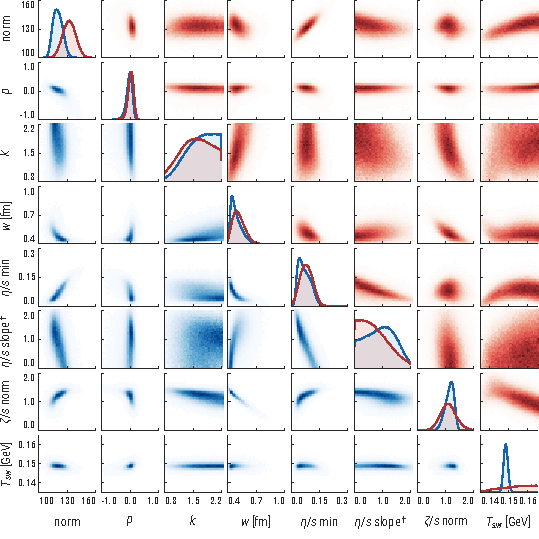
\includegraphics{posterior}};}
            \end{tikzpicture}
        \end{column}
        \begin{column}{1 cm}
            \centering
            \rotatebox[origin=c]{-90}{\scriptsize \only<1>{\color{pyred}} 
            \only<2->{\color{pyred!40}} Calibrated to charged particles}
            \hspace{0.4 cm}
        \end{column}
    \end{columns}

    \only<2>{
    \begin{tikzpicture}[remember picture, overlay]
        \filldraw [draw=almostblack, fill=almostblack, overlay, opacity=0.1, anchor=center] (current page.south west) rectangle (\paperwidth,\paperwidth);
        \node[inner sep=0pt, yshift=1cm, overlay] (node1) at (current page.center) {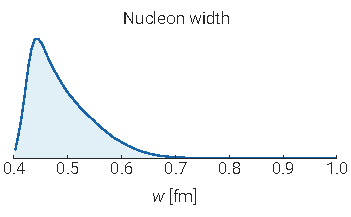
\includegraphics{posterior_w}};
        \node[inner sep=0pt, below=2ex of node1.south, anchor=north] {
            \begin{tcolorbox}[width=0.552\textwidth, boxrule=0pt, colback=white, colframe=almostblack, sharp corners]
                \scriptsize \centering
                Gaussian nucleon thickness: \medskip \\
                $T_p(x,y) = \frac{1}{2 \pi w^2} e^{-(x^2 +y^2)/(2w^2)}$
            \end{tcolorbox}
        };
    \end{tikzpicture}}

\end{frame}

\end{document}
